\documentclass{article}

\usepackage{polski} % Pozwala na użycie polskiego. Ustawia między innymi fontenc na T1
\usepackage[utf8]{inputenc} % Informuje o kodowaniu

\usepackage{graphicx}
\graphicspath{ {./Obrazy/} }

\usepackage{textcomp} % Znaki specjalne takie jak ~
\usepackage{listings} % Fragmenty kodu

\title{Laboratorium sieci komputerowych -- C1 \\ Wirtualizacja i zdalny dostęp}
\author{Krzysztof Dąbrowski gr. 3}
\date{\today}

\begin{document}
\maketitle{}
\tableofcontents{}
\newpage

\section{Wstęp}
Laboratorium \texttt{c1} było podzielone na dwa spotkania. Celem pierwszego było zapoznanie się z mechanizmem tworzenia i korzystania z maszyn wirtualnych. Podczas drugiego spotkania możliwe było przećwiczenie zdalnego korzystania z interfejsów graficznych.

\section{Wirtualizacja}
Technologia wirtualizacji umożliwia by komputer symulował działanie wybranej maszyny tak jakby była fizycznym komputerem. System przeprowadzający symulację nazywany jest \textit{gospodarzem}, natomiast system symulowany nazywany jest \textit{gościem}.

Do tworzenia i zarządzania wirtualnymi maszynami gospodarz potrzebuje specjalnego programu -- wirtualtizatora.

\paragraph{Powszechnie stosowane wirtualizatory:}
\begin{itemize}
    \item KVM
    \item Virtual box
    \item Bhyve
    \item Hyper-V
    \item VMWare
\end{itemize}

\subsection{Instalacja wirtualizatora}
Podczas zajęć wykorzystywany był wirtualizator Virtaul box. W celu automatyzacji instalacji programu napisany został skrypt.
\begin{lstlisting}[language=sh]
    #!/bin/sh
    sudo apt-get update
    sudo apt install virtualbox
    sudo apt install virtualbox-ext-pack 
\end{lstlisting}
Instaluje on program Virtual box oraz związaną z nim paczkę rozszerzeń. 

W celu możliwości korzystania z tego skryptu z dowolnego katalogu należało dopisać folder ze skryptem do zmiennej \texttt{PATH}. By ta zmiana dokonywała się automatycznie za każdym razem trzeba dodać eksport zmiennej \texttt{PATH} to pliku konfiguracyjnego \texttt{.zshenv}. Dzięki temu interpreter poleceń zsh automatycznie ustawi zmienną.

\subsection{Wirtualna maszyna}
Program Vitrual box oferuje bogaty interfejs graficzny. Za jego pomocą utworzona została maszyna o typie -- FreeBSD, ilości dostępnego ramu -- 1GB oraz bez dysku twardego.

Po przejściu przez początkowe ekrany kreacji możliwe było dodanie interfejsu do podłączenia płyty. Do wirtualnej stacji płyt został włożony dysk .iso z obrazem \textit{liveCD} systemu FreeBSD. Płyta tego typu umożliwia start systemu bez dysku twardego. Wszystkie informacje przechowywane są w pamięci RAM.

\paragraph{Wczytanie systemu z sieci} było ostatnim zadaniem przewidzianym na \\ pierwsze spotkanie. By umożliwić start systemu z sieci należało ustawić konfigurację sieciową gościa. Kluczowe było wybranie \textbf{połączenia mostkowego} by umożliwić dwukierunkową komunikację gościa z siecią. \\ Pozostałe ustawienia wyglądały następująco:
\begin{figure}[h]
    \centering
    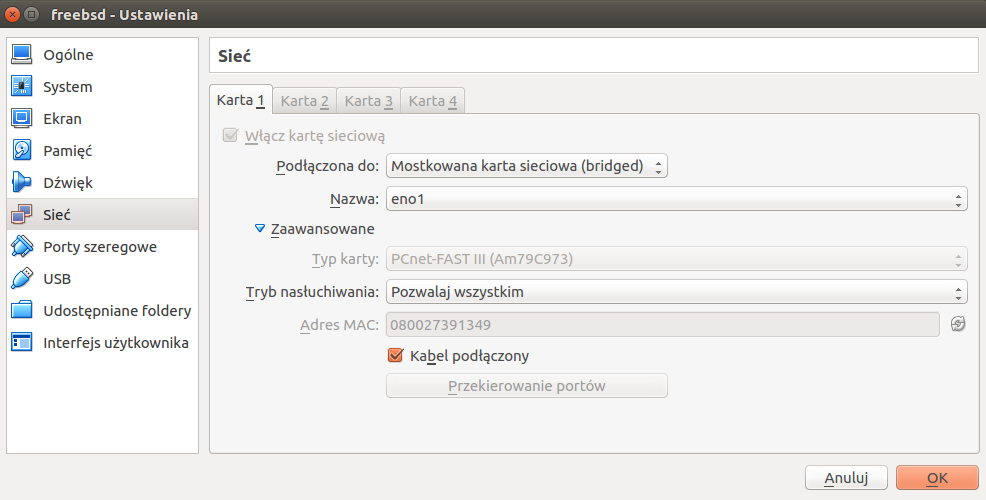
\includegraphics[width=0.95\textwidth]{ustawienia_karty_sieciowej}
\end{figure}

\end{document}